\subsection{Постановка задачи}
1.4. Реализовать метод вращений в виде программы, задавая в качестве входных данных матрицу и точность вычислений. Используя разработанное программное обеспечение, найти собственные значения и собственные векторы симметрических матриц. Проанализировать зависимость погрешности вычислений от числа итераций. 

{\bfseries Вариант:} 19
\begin{equation}
      \begin{pmatrix}
        -8 & 9 & 6\\
        9 & 9 & 1\\
        6 & 1 & 8
      \end{pmatrix}
\end{equation}
\pagebreak

\subsection{Результаты работы}

\begin{figure}[h!]
\centering
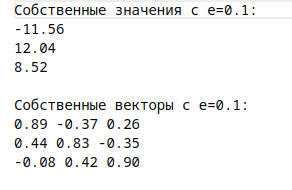
\includegraphics[width=.5\textwidth]{lab1.4}
\caption{Вывод в консоли}
\end{figure}
\pagebreak

\vfill

\subsection{Исходный код}

\lstinputlisting[title=\texttt{Lab1.4.cpp}]{../stud/saifullin/task1.4/Lab1.4.cpp}
\pagebreak
